\chapter{Modelización de la tarea de aprendizaje} \label{ch:tarea_aprendizaje}

\section{Planteamiento del problema} \label{seq:planteamiento_problema}

La tarea de aprendizaje que consideramos es la de \textbf{clasificación de imágenes}. El uso de redes convolucionales profundas ha supuesto un gran avance a la hora de resolver esta tarea. Nos centraremos en modelar redes convolucionales (profundas y no profundas) para clasificar imágenes.

Dado un elemento $X = (\nv{x_1}, \ldots, \nv{x_N})$, donde $\nv{x_i} \in \R^s \ \forall i \in \deltaset{N}$, queremos clasificarlo en alguna de las etiquetas $\mathcal{Y} = \{1, \ldots, Y \} = \deltaset{Y}$. Con esto, podemos ver que los datos de entrada viven en el espacio

\begin{equation}
	\mathcal{X} := \R^s \times \overset{N}{\ldots} \times \R^s = (\R^s)^N
\end{equation}

Esta representación de los datos de entrada es natural en muchos escenarios. En el caso de las imágenes, podemos considerar cada vector $\nv{x_i}$ como un conjunto de \textit{pixels} de la imagen (parche o \textit{patch}). Por la estructura local de las imágenes, cada vector de \textit{pixels} debería contener un vecindario de \textit{pixels}, es decir, \textit{pixels} adyacentes. Puede ocurrir que existan \textit{pixels} que aparezcan en más de un parche. Las imágenes contienen información en los colores que contiene cada píxel, pero también en la posición de los píxeles. Por ejemplo, si permutamos aleatoriamente las posiciones de los píxeles de una imagen, como hacemos en \imgref{img:desordenar_pixeles_repetida_mates}, esta imagen pierde completamente el sentido. A esto nos referimos cuando hablamos de estructura local de la imagen. Una forma natural de generar estos parches a partir de las imágenes consiste en tomar $\nv{x_i}$ como la fila o columna $i$-ésima de la imagen.

\begin{figure}[!hbtp]
	\centering
	\ajustarsubcaptions
	\begin{subfigure}[t]{0.45\textwidth}
		\centering
		
\includegraphics[width=0.9\linewidth]{informatica/ejemploperm_normal}
		\caption{Imagen original}
	\end{subfigure}
	\begin{subfigure}[t]{0.45\textwidth}
		\centering
		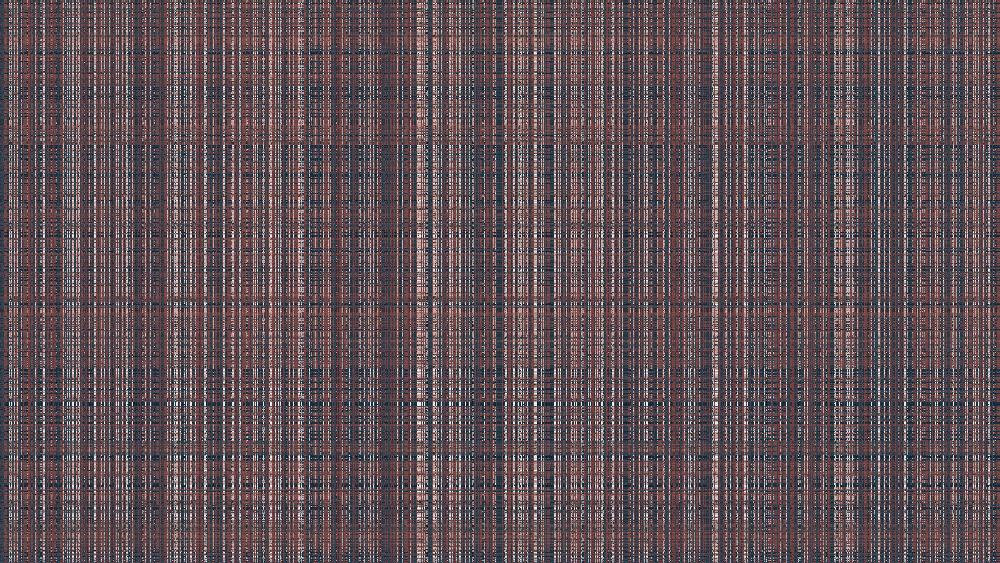
\includegraphics[width=0.9\linewidth]{informatica/ejemploperm_permutada}
		\caption{Imagen original tras aplicar una permutación aleatoria de las posiciones de los píxeles}
	\end{subfigure}
	\caption{Tenemos que considerar la estructura local de la imagen. La posición de los píxeles y su vecindario contiene una información fundamental de la que no podemos prescindir. Por tanto, los parches deben contener vecindarios de píxeles, aunque tengamos distintas estrategias para escoger estos vecindarios.}
	\label{img:desordenar_pixeles_repetida_mates}
\end{figure}

Para decidir la etiqueta de un elemento, consideramos $Y$ \textbf{funciones de puntuación}:

\begin{equation}
	\conjunto{h_y: \mathcal{X} \to \R \dspace / \dspace y \in \mathcal{Y}}.
\end{equation}

Con esto, dado un elemento $X \in \mathcal{X}$, lo clasificaremos buscando la etiqueta cuya función de puntuación sea máxima, es decir:

$$\hat{y} := \underset{y \in \mathcal{Y}}{argmax} \dspace h_y(X)$$

Por tanto, nuestro \textbf{espacio de hipótesis} es el conjunto de funciones $\Gamma := \conjunto{f: \mathcal{X} \to \R}$. Tanto en la práctica con modelos de \textit{machine learning}, como en nuestras dos modelizaciones, trabajamos en un subconjunto $\tilde{\Gamma} \subseteq \Gamma$ de funciones de puntuación, implementables o bien por el modelo de \textit{machine learning} o bien por nuestra modelización teórica.

\section{Espacio de hipótesis general}
\todo{JMERI: leer de nuevo esta sección completa, porque es muy liosa, repito cosas, introduzco cosas donde no debería. Mirar los contenidos que he borrado}

Nuestro objetivo en esta sección es justificar la elección de las funciones $h_y$ que conformarán el espacio de hipótesis sobre el que trabajaremos. En la \sectionref{sec:repr_funciones_puntuacion} mostramos cuál es la elección final basada en el desarrollo previo. Usaremos ciertos hechos básicos sobre análisis funcional que hemos introducido en la \sectionref{sec:preliminares_funcional}.

\subsection{Planteamiento para construir el espacio de hipótesis} \label{sec:justificacion_func_repr}

Recordemos que, como ya hemos introducido en la \sectionref{seq:planteamiento_problema}, nuestros datos de entrada viven en el espacio $\mathcal{X} = (\R^s)^N$. Para cada entrada $X \in \mathcal{X}$ tomamos como salida la etiqueta $\hat{y} \in \mathcal{Y}$ que maximice su función de puntuación asociada, es decir:

\begin{equation}
	\hat{y} := \underset{y \in \mathcal{Y}}{argmax} \dspace h_y(X)
\end{equation}

Por lo tanto, buscamos \textbf{construir un espacio de hipótesis} $\mathcal{H} \subseteq L^2((R^s)^N)$ donde elegir nuestras funciones de puntuación. Dicha elección influirá en los modelos de aprendizaje que podamos desarrollar.

En la \sectionref{subs:caracterizaciones_familias_funciones} hemos visto que, tomando $\{f_d(\nv{x}): d \in \N\} \subseteq L^2(R^s)$ de forma que sea total, tenemos $\varepsilon$-aproximación en $L^2(R^s)$ con combinaciones lineales finitas. Es más, en este caso el conjunto inducido de funciones producto punto a punto, $\{(\nv{x_1}, \ldots, \nv{x_n}) \mapsto \prod_{i = 1}^N f_{d_i}(\nv{x_i}) \}_{d_1, \ldots, d_N \in \N}$, también será total y, por lo tanto, tendremos $\varepsilon$-aproximación en $L^2((R^s)^N)$. A las funciones $\conjunto{f_d: \R^s \to \R: d \in \N}$ las llamaremos \textbf{funciones de representación}.

En resumen, buscamos tomar una elección de funciones $\{f_d(\nv{x}): d \in \N\} \subseteq L^2(R^s)$ que sea total, para así inducir un conjunto de funciones producto punto a punto total. Y con esto, dada cualquiera $h_y \in L^2((R^s)^N$, podemos aproximar dicha función de puntuación arbitrariamente bien ($\epsilon$-aproximación dada en la \propref{prop:conjuntos_totales_epsilon_aproximacion}) con combinaciones lineales finitas.

\subsection{Implementación del planteamiento}

Reflejamos este planteamiento de forma que sea más manejable en la búsqueda de un modelo matemático. Queremos expresar de forma cómoda y manejable la aproximación por combinaciones lineales finitas a partir de las funciones de puntuación $\conjunto{f_d: \; d \in \N}$.

Para ello, consideraremos tensores formales $\mathcal{A}^y \in \espaciotensores{N}{\N}$. Esto es, tensores con $N$ modos, cada modo con una dimensión infinita numerable (podemos considerar que tenemos $N$ sucesiones). El papel de estos tensores formales será el de almacenar los coeficientes de la combinación lineal finita dada por \eqref{eq:conjuntos_totales_epsilon_aproximacion}. Como esa combinación lineal es finita, nuestro tensor formal tendrá todas las entradas nulas, salvo un conjunto finito. Necesitamos usar tensores formales porque tenemos que elegir qué funciones usamos de un conjunto numerable. Y con esto llegamos a:

\begin{equation} \label{eq:hipotesis_en_general}
	h_y(\nv{x_1}, \ldots, \nv{x_N}) \approx \sum_{d_1, \ldots, d_N \in \N} A^y_{d_1, \ldots, d_N} \prod_{i = 1}^N f_{d_i}(\nv{x_i})
\end{equation}

\begin{observacion}

	La idea de cercanía que denota $\approx$ viene perfectamente dada por \eqref{eq:conjuntos_totales_epsilon_aproximacion}. Además, y como ya hemos comentado, el número de entradas no nulas del tensor dependerá del valor de $\varepsilon$. Pero esta ecuación no da problemas porque la relación entre estos dos elementos viene implícita.

\end{observacion}

Por tanto, \eqref{eq:hipotesis_en_general} \textbf{define un modelo universal}, puesto que cualquier función de representación $h_y$ puede ser aproximada arbitrariamente bien con combinaciones lineales en nuestro conjunto de funciones total.

\subsection{Elección de la familia de funciones de representación}

Como hemos justificado, tenemos que escoger una familia paramétrica de funciones de representación que sea numerable y además total, es decir:

\begin{equation}
	\mathcal{F} = \conjunto{ f_{\theta}: \R^s \to \R: \; \theta \in \Theta, \; \# \Theta = \# \N }
\end{equation}

Las opciones más usadas en la práctica del aprendizaje automático son:

\begin{enumerate}
	\item Wavelets
	\item Funciones de base radial (RBF), en concreto, la Gaussiana con matriz de covarianzas diagonal:

	      \begin{equation}
		      f_\theta(\nv{x}) = \mathcal{N}(\nv{x}; \nv{\mu}, diag(\nv{\sigma^2}))
	      \end{equation}

	      donde $\theta = (\nv{\mu}, \nv{\sigma^2})$ con $\nv{\mu} \in \R^s$, $\nv{\sigma^2} \in \R^s_+$

    \item Neuronas: véase la \sectionref{subsubs:capa_totalmente_conectada}


\end{enumerate}

Como veremos más adelante al especificar nuestro modelo, podemos tomar un conjunto finito de funciones de representación que sea total, es decir, podemos tomar $\{f_{\theta_d}: d \in \deltaset{M}\} \subseteq L^2(\R^s)$ total en la ecuación \eqref{eq:hipotesis_en_general}. Con ello, ahora es suficiente tomar $\mathcal{A}^y \in \espaciotensores{N}{M}$, llegando a:

\begin{equation}
	h_y(\nv{x_1}, \ldots, \nv{x_N}) = \sum_{d_1, \ldots, d_N = 1}^{M} \mathcal{A}^y_{d_1, \ldots, d_N} \prod_{i = 1}^N f_{\theta_{d_i}}(\nv{x_i})
\end{equation}

\begin{observacion}

	Nada nos impide tomar la familia de funciones $\{f_{\theta_d}: d \in \deltaset{M}\}$ de forma que sea también linealmente independiente. Como comentamos en \customref{sec:preliminares_funcional}, la familia de funciones producto punto a punto inducida,

	\begin{equation}
		\{ (\nv{x_1}, \ldots, \nv{x_N}) \mapsto \prod_{i = 1}^N f_{d_i}(\nv{x_i}): d_i \in \N \}
	\end{equation}

	será también linealmente independiente, por lo que será una base del espacio $L^2((R^s)^N)$. Y por tanto, una función de puntuación $h_y$ \textbf{determina unívocamente un tensor de coeficientes} $\mathcal{A}^y$.

\end{observacion}

\begin{observacion}
	Usamos la notación $\sum_{d_1, \ldots, d_N = 1}^{M}$ para denotar $\sum_{d_1 = 1}^{M} \sum_{d_2 = 1}^{M} \ldots \sum_{d_N = 1}^{M}$.
\end{observacion}

\subsection{Representación de las funciones de puntuación} \label{sec:repr_funciones_puntuacion}

Por todo esto, las funciones de puntuación vendrán dadas de la forma:

\begin{equation} \label{eq:puntuacion_general}
	h_y(\nv{x_1}, \ldots, \nv{x_N}) = \sum_{d_1, \ldots, d_N = 1}^{M} \mathcal{A}^y_{d_1, \ldots, d_N} \prod_{i = 1}^N f_{\theta_{d_i}}(\nv{x_i})
\end{equation}

Las funciones $f_{\theta_1}, \ldots, f_{\theta_M}: \R^s \to \R$ son las \textbf{funciones de representación}, que como ya hemos comentado, suelen ser \textit{Wavelets}, funciones de base radial (\textit{RBF}) o neuronas.

El tensor $\mathcal{A}^y$ será el \textbf{tensor de coeficientes}. Por la sumatoria en \eqref{eq:puntuacion_general}, es claro que tiene orden $N$ y dimensión $M$ en cada modo. Es decir, $\mathcal{A} \in \espaciotensores{N}{M}$.

Por lo tanto, la tarea de aprendizaje consistirá en optimizar los valores de los parámetros $\theta_1, \ldots, \theta_M$ y los valores de los tensores de coeficientes $\mathcal{A}^1, \ldots, \mathcal{A}^Y$.

\begin{observacion}
	Por lo comentado previamente, estamos trabajando con un conjunto de funciones de representación $\conjunto{f_d: \; d \in \deltaset{M}}$ total y linealmente independiente. Por tanto, el conjunto de funciones producto punto a punto también será total y linealmente independiente (\customref{prop:conservacion_totalidad_indp_lineal_func_prod}):

	\begin{equation}
		\conjunto{(\nv{x_1}, \ldots, \nv{x_N}) \mapsto \prod_{i = 1}^{N} f_{\theta_{d_i}} (\nv{x_i}): \dspace d_i \in \deltaset{M} \dspace \forall i \in \deltaset{N} }
	\end{equation}


	Sabemos entonces que esta familia de funciones actuará como una \entrecomillado{base} del espacio $L^2((\R^s)^N)$. Y por lo tanto podemos pensar que el tensor $\mathcal{A}^y$ nos da los coeficientes de la función de puntuación $h_y$ en dicha \entrecomillado{base}.
\end{observacion}
\todo{Comentario de JMeri: Esto está repetido varias veces. Tengo que repasar toda la sección}

\begin{observacion}
	Como $\mathcal{A} \in \espaciotensores{N}{M}$, tenemos que optimizar el valor de $M^N$ valores reales a través del proceso de aprendizaje. Esto supone un reto, que \textbf{motiva el uso de los dos modelos}, que se basarán en descomposiciones tensoriales para que el aprendizaje del tensor de coeficientes sea más factible.
\end{observacion}

\subsection{Capa de representación} \label{subs:capa_de_representacion}

En \eqref{eq:puntuacion_general} estamos usando las mismas funciones de representación $f_{\theta_1}, \ldots, f_{\theta_M}: \R^s \to \R$ para todas las funciones de puntuación $h_y$. Lo único que cambia entre las distintas funciones de puntuación es el tensor de coeficientes $\mathcal{A}^y$. Nótese además que en la ecuación \refeq{eq:puntuacion_general}, los vectores de entrada $\nv{x_i}$ solo participan en el producto que involucra computar $f_{\theta_{d_i}}(\nv{x_i})$. Por tanto, podemos considerar un paso inicial, que será compartido en los dos modelos que más adelante introduciremos, consistente en computar los valores:

$$\{f_{\theta_d}(\nv{x_i}): \; d \in \deltaset{M},\ i \in \deltaset{N} \}$$

Una vez que hayamos computado esos $M \cdot N$ valores, ya no necesitamos los valores $\nv{x_i}$ para nada más. Con esto, es natural considerar que nuestro modelo tenga una primera capa que compute esos valores. Podemos considerar dicha capa como una \textbf{primera capa convolucional} con $M$ canales, a la que llamaremos \textbf{capa de representación}. Por tanto, cada parche de entrada $\nv{x_i} \in \R^s$ acaba siendo representando por un descriptor de longitud $M$.

Y como ya hemos comentado, estamos usando las mismas funciones de representación para las $Y$ funciones de puntuación. Por tanto, fijados los parámetros $\theta_i$, en todas las funciones de puntuación la capa de representación será la misma.

El siguiente diagrama muestra gráficamente cómo actúa la capa de representación, calculando los $N \cdot M$ coeficientes reales que componen dicha capa:

\begin{figure}[!hbtp]
	\centering
	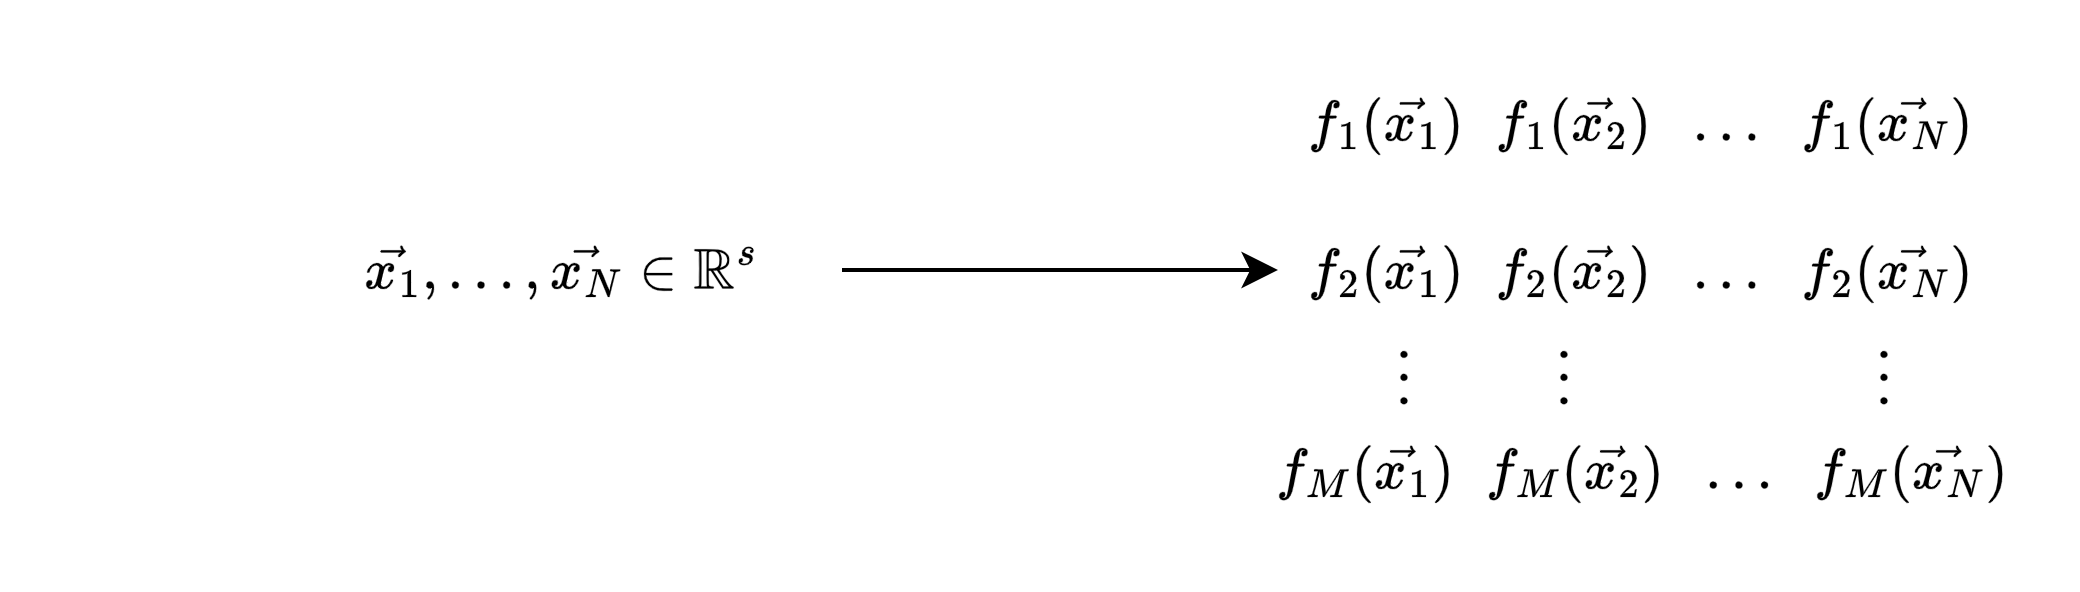
\includegraphics[width=0.8\textwidth]{matematicas/computo_capa_representacion}
	\caption{Ejemplo gráfico sobre cómo actúa la capa de representación. A partir de $N$ parches en $\R^s$, acabamos con $N \cdot M$ coeficientes reales}
\end{figure}


\subsection{Ejemplo de cómputo} \label{ejemplo:funcion_puntuacion}

Supongamos que trabajamos con $N = 3, M = 2$. En este caso, una imagen de entrada se compone de los vectores $\nv{x_1}, \nv{x_2}, \nv{x_3} \in \R^s$ (no estamos interesados en el valor de $s \in \N$). Y tenemos dos funciones de representación $f_1, f_2: \R^s \to \R$.

El primer paso es computar la capa de representación, que son los $N \cdot M$ coeficientes reales dados por:

\begin{equation}
	\begin{split}
		f_1(\nv{x_1}), f_1(\nv{x_2}), f_1(\nv{x_3}) \\
		f_2(\nv{x_1}), f_2(\nv{x_2}), f_2(\nv{x_3})
	\end{split}
\end{equation}

Y con esto ya podemos expresar nuestra función de puntuación:

\begin{equation}
	\begin{split}
		h_y(\nv{x_1}, \ldots, \nv{x_N}) &= \sum_{d_1, d_2, d_3 = 1}^{2} \mathcal{A}^y_{d_1 d_2 d_3} \prod_{i = 1}^3 f_{d_i}(\nv{x_i}) = A_{111} \; f_1(\nv{x_1}) \; f_1(\nv{x_2}) \; f_1(\nv{x_2}) + A_{112} \; f_1(\nv{x_1}) \; f_1(\nv{x_2}) \; f_2(\nv{x_2}) + \\
		\cdots &+ A_{321} \; f_3(\nv{x_1}) \; f_2(\nv{x_2}) \; f_1(\nv{x_2}) + A_{333} \; f_3(\nv{x_1}) \; f_3(\nv{x_2}) \; f_3(\nv{x_3})
	\end{split}
\end{equation}

Queda claro que el tensor $\mathcal{A}^y$ contiene los coeficientes que realizan una combinación lineal sobre todos los posibles productos de nuestros $N \cdot M$ valores reales de la capa de representación.

\section{Resumen}

Buscamos resolver una tarea de clasificación. Es decir, buscamos clasificar imágenes en una de las etiquetas $\mathcal{Y} := \{1, \ldots, Y\} = \deltaset{Y}$. Las imágenes de entrada se dividen en parches. Esto es, una imagen viene dada por $N$ vectores $x = (\nv{x_1}, \ldots, \nv{x_N}), \dspace \nv{x_i} \in \R^s \dspace \forall i \in \deltaset{N}$. Al disponer de $M$ funciones de representación, cada vector $\nv{x_i}$ acabará siendo \textbf{representado} por un descriptor de longitud $M$, es decir:

\begin{equation}
	\nv{x_i} \to (f_1(\nv{x_i}), \ldots, f_M(\nv{x_i})) \in \R^M
\end{equation}

Para resolver la tarea de clasificación, buscamos aprender $Y$ funciones de puntuación $h_y$. Para ello, tomamos los $N \cdot M$ coeficientes resultado de tomar $N$ descriptores de longitud $M$. La función de puntuación $h_y$ es el resultado de combinar linealmente los $M^N$ posibles productos de los $N \cdot M$ coeficientes. La combinación lineal se describe con los coeficientes de $\mathcal{A}^y \in \espaciotensores{N}{M}$.

Las dos arquitecturas que introduciremos más adelante son el resultado de factorizar el tensor de coeficientes $\mathcal{A}^y$ con distintas descomposiciones. Ambas incorporan conceptos claves en la práctica del aprendizaje automático, como la localidad, coeficientes compartidos y \textit{pooling}, que explicaremos más adelante.
